\def\mytitle{MATRICES USING PYTHON}
\def\myauthor{TOTLI.VARSHA REDDY}
\def\contact{varshareddy724@gmail.com}
\def\mymodule{Future Wireless Communication (FWC)}
\documentclass[10pt, a4paper]{article}
\usepackage[a4paper,outer=1.5cm,inner=1.5cm,top=1.75cm,bottom=1.5cm]{geometry}
\twocolumn
\usepackage{graphicx}
\graphicspath{{./images/}}
\usepackage[colorlinks,linkcolor={black},citecolor={blue!80!black},urlcolor={blue!80!black}]{hyperref}
\usepackage[parfill]{parskip}
\usepackage{lmodern}
\usepackage{tikz}
 \usepackage{physics}
%\documentclass[tikz, border=2mm]{standalone}
\usepackage{karnaugh-map}
%\documentclass{article}
\usepackage{tabularx}
\usepackage{circuitikz}
\usetikzlibrary{calc}
\usepackage{amsmath}
\usepackage{amssymb}
\renewcommand*\familydefault{\sfdefault}
\usepackage{watermark}
\usepackage{lipsum}
\usepackage{xcolor}
\usepackage{listings}
\usepackage{float}
\usepackage{titlesec}
\providecommand{\mtx}[1]{\mathbf{#1}}
\titlespacing{\subsection}{1pt}{\parskip}{3pt}
\titlespacing{\subsubsection}{0pt}{\parskip}{-\parskip}
\titlespacing{\paragraph}{0pt}{\parskip}{\parskip}
\newcommand{\figuremacro}[5]

\begin{document}

\title{\mytitle}
\author{\myauthor\hspace{1em}\\\contact\\FWC22036\hspace{6.5em}IITH\hspace{0.5em}\mymodule\hspace{6em}ASSIGN-4}
\date{}
 \maketitle
  %\begin{figure}
 \tableofcontents
\vspace{10mm}
   \section{Problem}
ABCD, DCFE and ABFE are parallelograms.Show that\\
ar(ADE)=ar(BCF).\\

   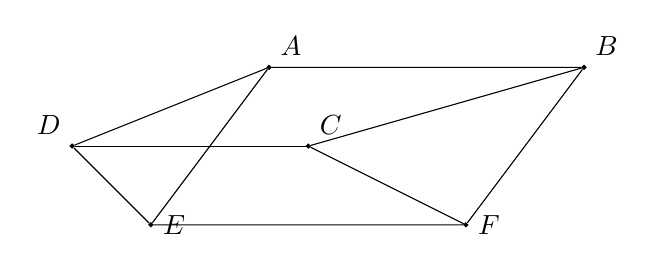
\begin{tikzpicture}
[scale=2,>=stealth,point/.style={draw,circle,fill = black,inner sep=0.5pt},]

%Triangle sides
\def\a{4.5}
\def\b{4.5}
\def\c{10}
\def\d{2.5}
%Labeling points
\node (A) at (0.75,1)[point,label=above right:$A$] {};
\node (B) at (2.75,1)[point,label=above right:$B$] {};
\node (C) at (1,0.5)[point,label= above right:$C$] {};
\node (D) at (-0.5,0.5)[point,label=above left:$D$] {};
\node (E) at (0,0)[point,label=right:$E$] {};
\node (F) at (2,0)[point,label=right:$F$] {};


%Drawing parallelogram ABCD
\draw (A) -- (B) --  (F) --(E)--(A);
\draw (E) -- (D) -- (A);
\draw (F) --(C) -- (B);
\draw (D) -- (C);

%\tkzMarkRightAngle[fill=blue!20,size=.2](B,C,D)
\end{tikzpicture}
\newline
   \textbf{Theory:}\\
    Parallelograms on the same base and in between the same parallels are equal in area.
Given: ABCD,DCFE and ABFE are parallelograms.\\
% Given $ AP\:  CR $ \\
\vspace{5mm}

 \section{Solution}
\textbf{To Prove:} Ar(ADE)=Ar(BCF) \\
parallelogram ABCD  lies  between same parallel lines AD and BC\\
\begin{center}
$\therefore$ AD = BC......(1)\\ 
\end{center}
 parallelogram DECF  lies  between same parallel lines DE and CF\\
\begin{center}
$\therefore$ DE = CF......(2)\\ 
\end{center}
 parallelogram ABEF  lies  between same parallel lines AE and FB\\
\begin{center}
$\therefore$ EA = FB
\end{center}
\begin{center}
In $\Delta$ADE , $\Delta$BCF\\
$\therefore$ AD = BC \\
$\therefore$ DE = CF \\
$\therefore$ EA = FB \\
$\therefore$ $\Delta$ ADE = $\Delta$ BCF\\
%$\therefore$ $\Delta$ ADE = $\Delta$ BCF\\

Hence, Proved \\
\
\\
\
\\
\end{center}
\vspace{3mm}
\textbf{Termux commands :}
\begin{lstlisting}
python3 matrixline.py
\end{lstlisting}


The input parameters for this construction are 
\begin{center}
\begin{tabular}{|c|c|c|}
	\hline
	\textbf{Symbol}&\textbf{Value}&\textbf{Description}\\
	\hline
	a&4.5&EA\\
	\hline
	b&4.5&BC\\
	\hline
	c&10&CD\\
	\hline
	d&2.5&DE\\
	\hline
	${\theta}_1$& 25$\pi/180$&$ \angle $BC\\ 
	\hline
	${\theta}_2$& 120$\pi/180$&$ \angle $DE\\ 
	\hline
	${\theta}_3$& 2$\pi/3$&$ \angle $AE\\ 
	\hline
	${\theta}_4$& 35$\pi/180$&$ \angle $CD\\ 
    \hline
	E&$\
	\begin{pmatrix}
		0 \\
		0 \\
	\end{pmatrix}$%
	&Point E\\
	\hline
\end{tabular}
\end{center}

\textbf{To Prove:} \\
  \begin{center}
  Ar(ADE)=Ar(BCF)\\
 v1=A-D\\
 v2=D-E\\
 \vspace{3mm}
 Area of the triangle $\Delta$ADE is given by \\
Ar($\Delta$ADE) =$\frac{1}{2}$$\norm{\vec{v1}\times\vec{v2}}$............(2)\\
\vspace{3mm}
v3=B-C\\
 v4=C-F\\
 \vspace{3mm}
  Area of the triangle $\Delta$BCF is given by \\
 Ar($\Delta$BCF) =$\frac{1}{2}$$\norm{\vec{v3}\times\vec{v4}}$...............(3)
 \end{center}
 \begin{center}
$\therefore$ Ar(ADE)=Ar(BCF)\\

\end{center}
\vspace{10mm}
The below python code realizes the above construction: \\

\url{https://github.com/KrishnaYadati/Assignments/tree/main/Matrix-line_ assignment/line_program}
 \section{Construction}
  \begin{center}
    \includegraphics[scale=1]{Documents/ABC.pdf}  
     Figure of Construction
   \end{center}
     
\bibliographystyle{ieeetr}
\end{document}
